\documentclass[12pt]{article}
\usepackage[utf8]{inputenc}
\usepackage{graphics}
\usepackage{graphicx}
\usepackage{float}
\usepackage{hyperref}

\title{Release plan}
\author{Thomas van Dongen, Koen Schilders}
\date{7 februari 2018}

\begin{document}


% De titelpagina
\begin{titlepage}
\maketitle
\end{titlepage}



% Hier worden alle branches beschreven
\section{Omschrijving per branch}
\begin{figure}[H]
	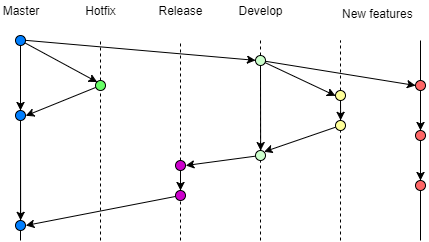
\includegraphics[width=\textwidth]{images/SOP6_Release.png}
	\caption{Het releaseplan.}
\end{figure}
\subsection{Master}
De master is de branch waar een geteste releases staan, bedoeld voor deployment. Het is mogelijk om een ontwikkelstraat op te zetten die een nieuwe commit naar de master automatisch build en deployed naar bijvoorbeeld de Appstore.
\subsection{Hotfix}
Als er een ernstige bug gevonden is in de master branch is het nodig om deze direct op te lossen. Een hotfix dient dan in de hotfix branch gemaakt te worden. Hiervoor wordt de build van de master gepulled, en een hotfix gemaakt. Vervolgens wordt deze naar de master gepushed als nieuwe versie.
\subsection{Release}
De build van develop wordt naar de release branch gepushed als deze compleet is. Het QA-team kan deze versie testen. Bugs kunnen in deze branch gefixed worden, waarna het QA-team deze versie opnieuw test. Als de versie de groene vlag krijgt, en er geen bugs gevonden zijn, kan de master branch deze versie pullen.
\subsection{Develop}
De develop branch wordt gebruikt als start punt voor het ontwikkelen van nieuwe features. Er wordt vanaf deze branch een nieuwe branch gemaakt en daar wordt verder op gewerkt. Er wordt dus nooit ontwikkeld op deze branch.
\subsection{New features}
Om er voor te zorgen dat het ontwikkelen van nieuwe branches goed verloopt maken we gebruik van feature branches. Elke nieuwe feature krijgt zijn eigen branch. Pas wanneer de feature af is wordt deze weer gemerged met de develop branch. De feature branch wordt na de merge verwijdert.



% Hier wordt het releaseplan gemaakt in Git beschreven
\pagebreak
\section{Releaseplan in Git}
\begin{figure}[H]
	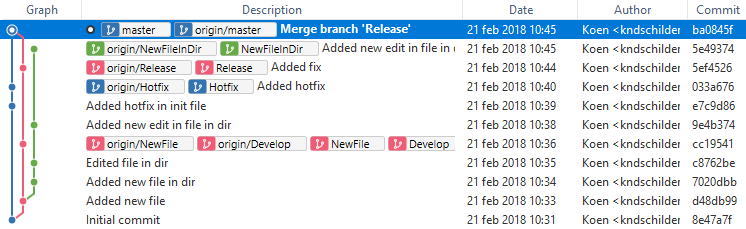
\includegraphics[width=\textwidth]{images/ReleasePlanInGit.png}
	\caption{Het releaseplan weergegeven in Sourcetree.}
\end{figure}
Het releaseplan beschreven in sectie 1 staat hierboven uitgewerkt in Sourcetree. In Sourcetree is het eenvoudig om een nieuwe branch aan te maken:

\begin{figure}[H]
	\centering
	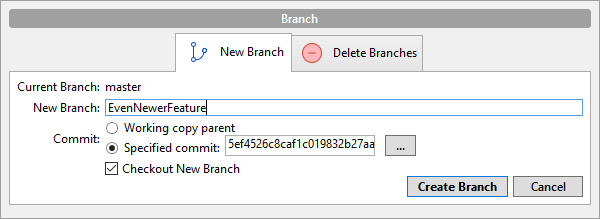
\includegraphics[width=\textwidth]{images/NewBranch.png}
\end{figure}

Er kan gekozen worden om de branch te beginnen vanaf een specifieke commit. Hiermee hebben we de opzet van het releaseplan nagemaakt.
\href{https://github.com/kndschilders/ReleasePlanGitTest}{Hier}
staat de volledige git repository. De branch 'NewFile' bestaat nog ter illustratie, maar zou in een echte production verwijderd moeten worden.

\end{document}